\documentclass{beamer}

\mode<presentation> {
  \usetheme{CambridgeUS}
  %\setbeamertemplate{footline} % To remove the footer line in all slides uncomment this line
  %\setbeamertemplate{footline}[page number] % To replace the footer line in all slides with a simple slide count uncomment this line
  %\setbeamertemplate{navigation symbols}{} % To remove the navigation symbols from the bottom of all slides uncomment this line
}

\usepackage{graphicx}
\usepackage{booktabs}
\usepackage{svg}

%----------------------------------------------------------------------------------------
%   TITLE PAGE
%----------------------------------------------------------------------------------------

\title[Project Object Recognition]{Learn pendulum feature from video}

\author{Louis THIRY, Marc SANSELME}
\institute[MVA]
{ENS-Cachan}
\date{\today}

\begin{document}

\begin{frame}
\titlepage
\end{frame}

\begin{frame}
\frametitle{Overview}
\tableofcontents
\end{frame}

%----------------------------------------------------------------------------------------
%   PRESENTATION SLIDES
%----------------------------------------------------------------------------------------

\section{Introduction}

\begin{frame}
\frametitle{Measure quantity with computer vision}
\begin{itemize}
  \item recording a video is really easy
  \item thanks to computer vison, kinematic informations (velocity, acceleration...) can be measuring
  \item thanks to mecanics, other quantities (mass, length...) can be deduced from these informations
\end{itemize}
$\rightarrow$ Proof of concept with a pendulum
\end{frame}

\begin{frame}
\frametitle{Simple pendulum}
\begin{figure}
  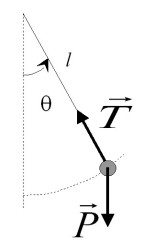
\includegraphics{pendule.jpg}
  \caption{Simple pendulum}
\end{figure}
\begin{align*}
  \ddot{\theta} + \frac{g}{l} \sin (\theta) = 0
\end{align*}
\end{frame}

\begin{frame}
\frametitle{Methodology}
\begin{itemize}
  \item Computer Vision : Deduce the angle sequence from a video
  \item Learning : Deduce the length from the angle sequence
\end{itemize}
\end{frame}

\section{From video to angle sequence}

\begin{frame}
\frametitle{CNN activation}
COMPLETER AVEC L'EXPLICATION DES ACTIVATIONS
\end{frame}

\begin{frame}
\frametitle{Activation examples}
DONNER DES EXEMPLES D'ACTIVATION
\end{frame}

\begin{frame}
\frametitle{Pendulum position detection with activations}
VIDEO DU PENDULE AVEC ACTIVATION
METHODE DE TRESHOLDING + SELECTION PAQUET + BARYCENTRE
\end{frame}

\begin{frame}
\frametitle{From pendulum position to pendulum angle}
METHODE LEAST SQUARES AVEC LA DISTANCE AUX RAYONS
\end{frame}

\section{From angle sequence to pendulum length}

\begin{frame}
\frametitle{One step integration of pendulum equation}
$\rightarrow$ pendulum length can be learnt from three angle
\end{frame}

\begin{frame}
\frametitle{Deduce the length}
Angle observations are noisy.
$\rightarrow$ average different length obtained on each three angle sequence
\end{frame}

\begin{frame}
\frametitle{Results}
\end{frame}

\begin{frame}
\frametitle{Extensions}
Double pendulum
\end{frame}

\end{document}
